%
% kapiza.tex
%
% (c) 2024 Prof Dr Andreas Müller
%
\begin{figure}
\centering
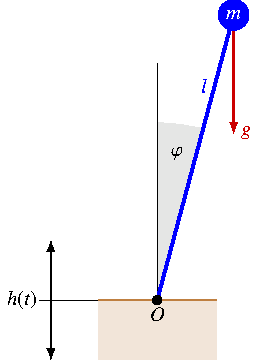
\includegraphics{chapters/090-mechanik/images/kapiza.pdf}
\caption{Das invertierte oder Kapiza Pendel besteht aus einer Masse $m$
am Ende einer masselosen Stange der Länge $l$, die drehbar im Punkt $O$
gelagert ist.
Die Koordinate $\varphi$ ist die Auslenkung des Pendels aus der Vertikalen.
Das Pendel unterliegt der Wirkung der Erdbeschleunigung $g$.
\label{buch:mechanik:lagrange:fig:kapiza}}
\end{figure}
